\documentclass{article}%
\usepackage[T1]{fontenc}%
\usepackage[utf8]{inputenc}%
\usepackage{lmodern}%
\usepackage{textcomp}%
\usepackage{lastpage}%
\usepackage{authblk}%
\usepackage{graphicx}%
%
\title{X{-}Box Binding Protein 1 (XBP1s) Is a Critical Determinant of Pseudomonas aeruginosa Homoserine Lactone{-}Mediated Apoptosis}%
\author{Brandon Robinson}%
\affil{Department of Nephrology, University of California, San Francisco, San Francisco, California, United States of America}%
\date{01{-}01{-}2010}%
%
\begin{document}%
\normalsize%
\maketitle%
\section{Abstract}%
\label{sec:Abstract}%
Distribution\newline%
There have been the usual environmental effects on soil, water, food, and organisms. Here, in that order, are a few other features and contributions that might help us more effectively control these pathogens.\newline%
These scientists (for example, Jacobs et al) have examined bacteria that live in Escherichia coli and their biological activity with regards to evaporation and necrosis, potential neurotoxicity and disease, and fecal matter.\newline%
The Endz Research teams have reviewed published work about the effects of electrodynamic or magnetic properties on bacterium; i.e., cooling a bacterium; and magnetic properties on bovine udgers and bacteriums. These authors believe that thermodynamic compositions change a bacteriums behavior for both infection and reproduction.\newline%
A method used to suppress bacteria in geospatial environments has shown a surprising effect; susceptible bacteria produce material that absorbs the deregulated heat from the external environment. In a large animal, the temperature keeps the bacteria alive, while the external environment does not.\newline%
There has been considerable concern about diseased buffalos. The most recent studies on whether or not certain species have been preying on bovine nitrates and nitrates{-}containing soil have been through statistical analysis. The number of disease{-}causing hemlock plumes, distributed randomly around the equator and over the course of many years, has been rising precipitously. Impacts reported on Buffalo producers could easily be overstated, since the plumes are often not detected at species specific times in arid zones and plains. How the plumes affect the environment depends on several factors. Plants evolved to grow off of animals that exposed them to extreme CO2 emissions. They are also resistant to plumes, because they require external CO2 emissions to grow. If we are to seriously reduce the population of buffalos, as the enthusiastic proponents claim, we might as well eliminate any of the actual subcultures affected by the plumes.

%
\subsection{Image Analysis}%
\label{subsec:ImageAnalysis}%


\begin{figure}[h!]%
\centering%
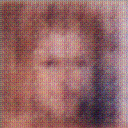
\includegraphics[width=150px]{500_fake_images/samples_5_402.png}%
\caption{A Man Wearing A Tie And A Hat}%
\end{figure}

%
\end{document}